\chapter{Case: Verified Koopa Troopa Movement}
\label{ch:case-koopa}


\section{Inleiding}

Deze eerste gevalstudie is geïnspireerd door de populaire Mario \cite{mario}
franchise van Nintendo \cite{nintendo}, in het bijzonder Super Mario Bros.
\cite{supmario}. Er zijn verschillende vijanden in het spel maar hier beperken
we ons tot de schildpadachtige Koopa Troopas. Zoals wel vaker voorkomt bevatten
vele van de Mariospellen zogenaamde \emph{glitches}, fouten die uitgebuit
kunnen worden om bepaalde acties uit te voeren die normaal moeilijk of
onmogelijk zijn. Zo is er bijvoorbeeld een fout met een Koopa Troopa waardoor
Mario aan het einde van het level over de vlag kan springen, dit is normaal
niet mogelijk. De precieze fout is moeilijk uit te leggen maar ze is mogelijk
omdat een Koopa Troopa als het ware onder het level kan rondlopen, dit is in
figuur \ref{koopaglitch} te zien. Deze fout is eigenlijk de precieze inspiratie
van deze gevalstudie.

\begin{figure}
  \centering
  \def\svgwidth{\textwidth}
  \import{figures/}{KoopaTroopaGlitch.pdf\string_tex}
  \caption{Onder Mario is nog net het hoofd van een Koopa Troopa te zien
           \cite{marioglitchyoutube}}
  \label{koopaglitch}
\end{figure}

De Koopa Troopas komen voor in twee kleuren: rood en groen. Ze lopen in één
richting tot ze een obstakel tegenkomen, dan keren ze om. Voor alle Koopa
Troopas is een muur een obstakel, enkel voor de rode Koopa Troopas is een
afgrond een obstakel. Dit heeft tot gevolg dat rode Koopa Troopas heen en weer
patrouilleren en groene Koopa Troopas eerder trapsgewijs naar beneden vallen
tot ze uit het beeld verdwijnen. Door deze regels uit te drukken in de types,
in plaats van in de spellogica, kunnen we een fout zoals die in figuur
\ref{koopaglitch} te zien is, voorkomen. In figuur \ref{kooparedgreen} zijn een
aantal voorbeeldpaden geïllustreerd.

\begin{figure}
  \centering
  \begin{subfigure}{0.49\textwidth}
    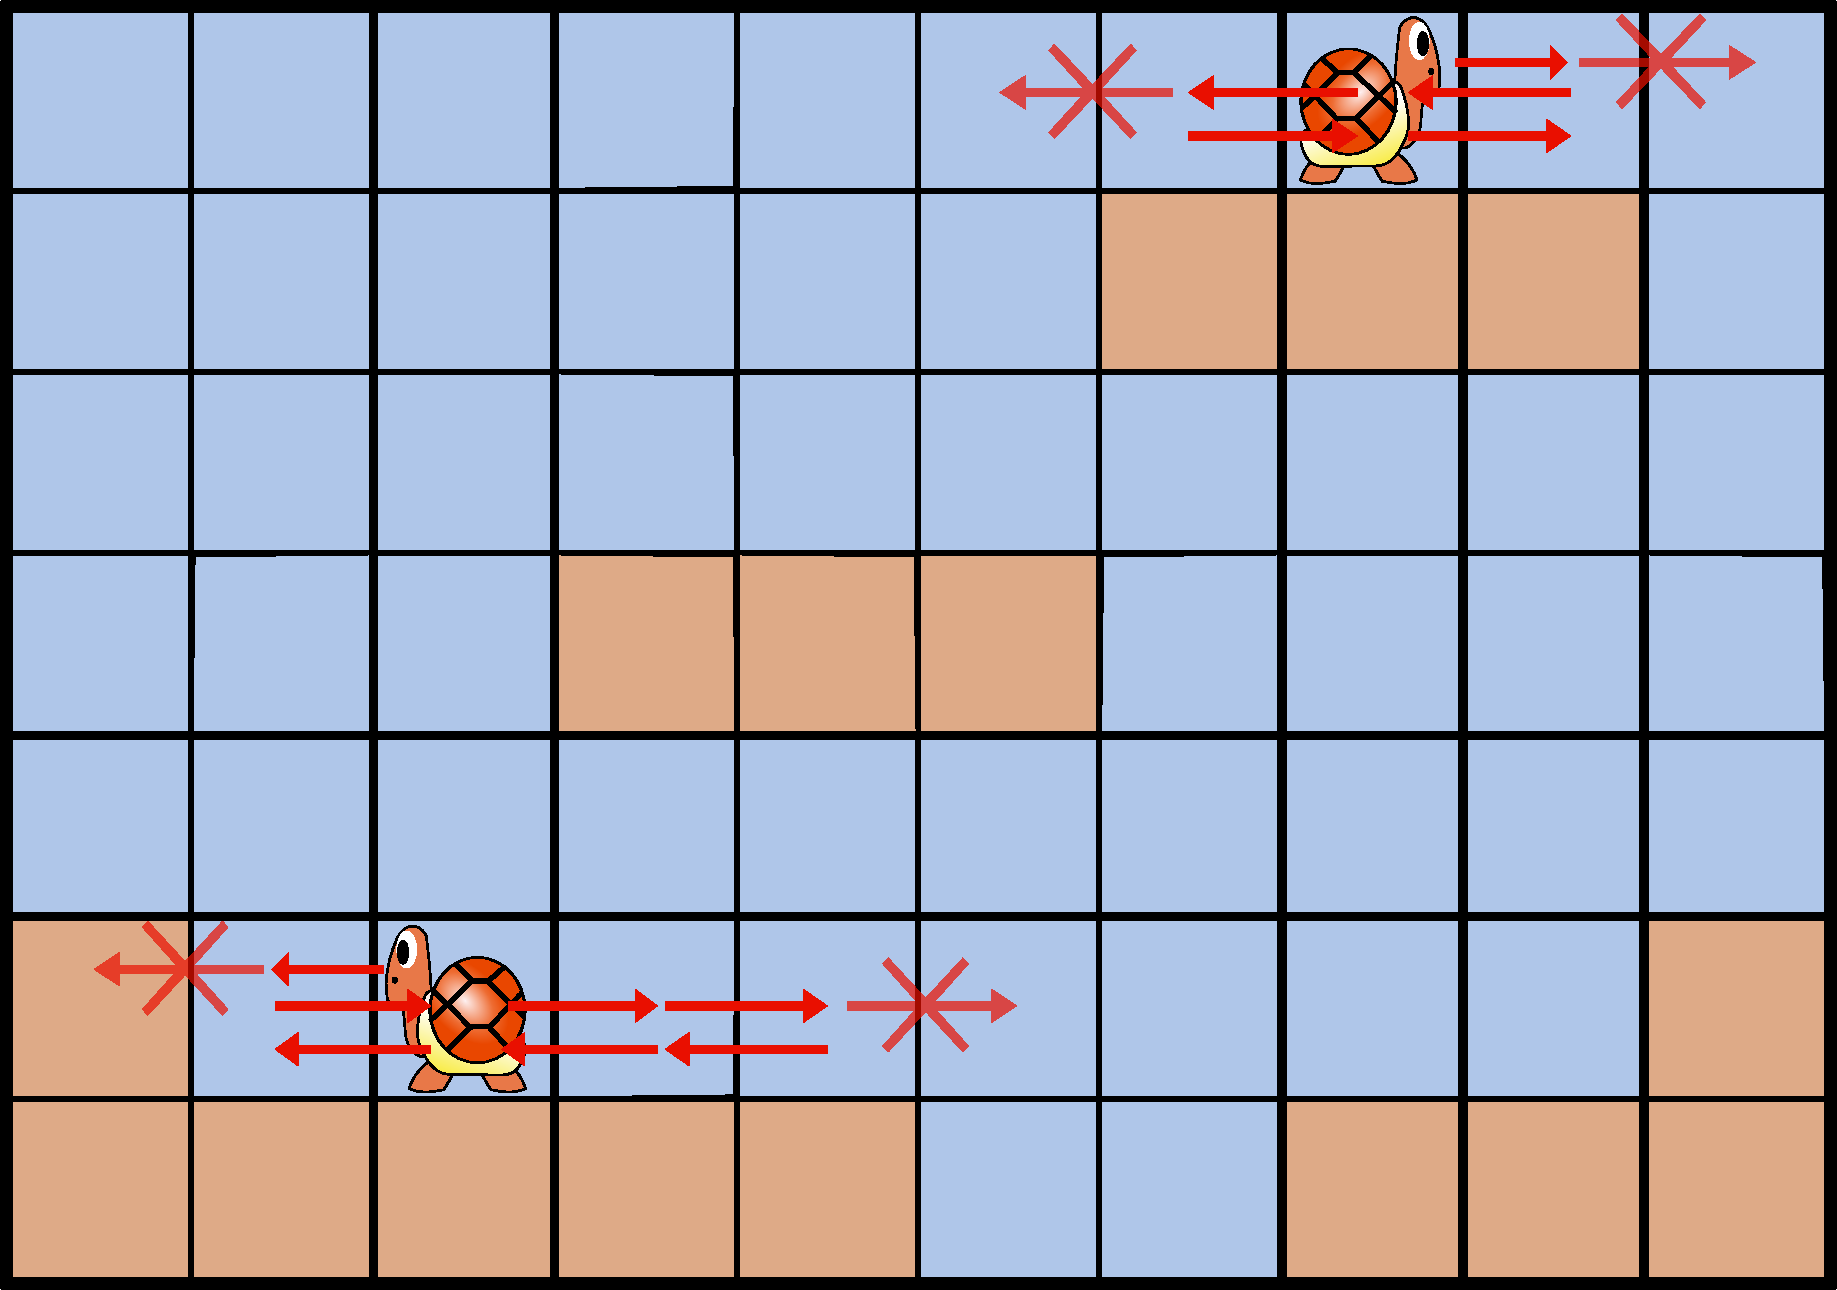
\includegraphics[width=\textwidth]{figures/koopatroopa-red}
  \end{subfigure}
  \begin{subfigure}{0.49\textwidth}
    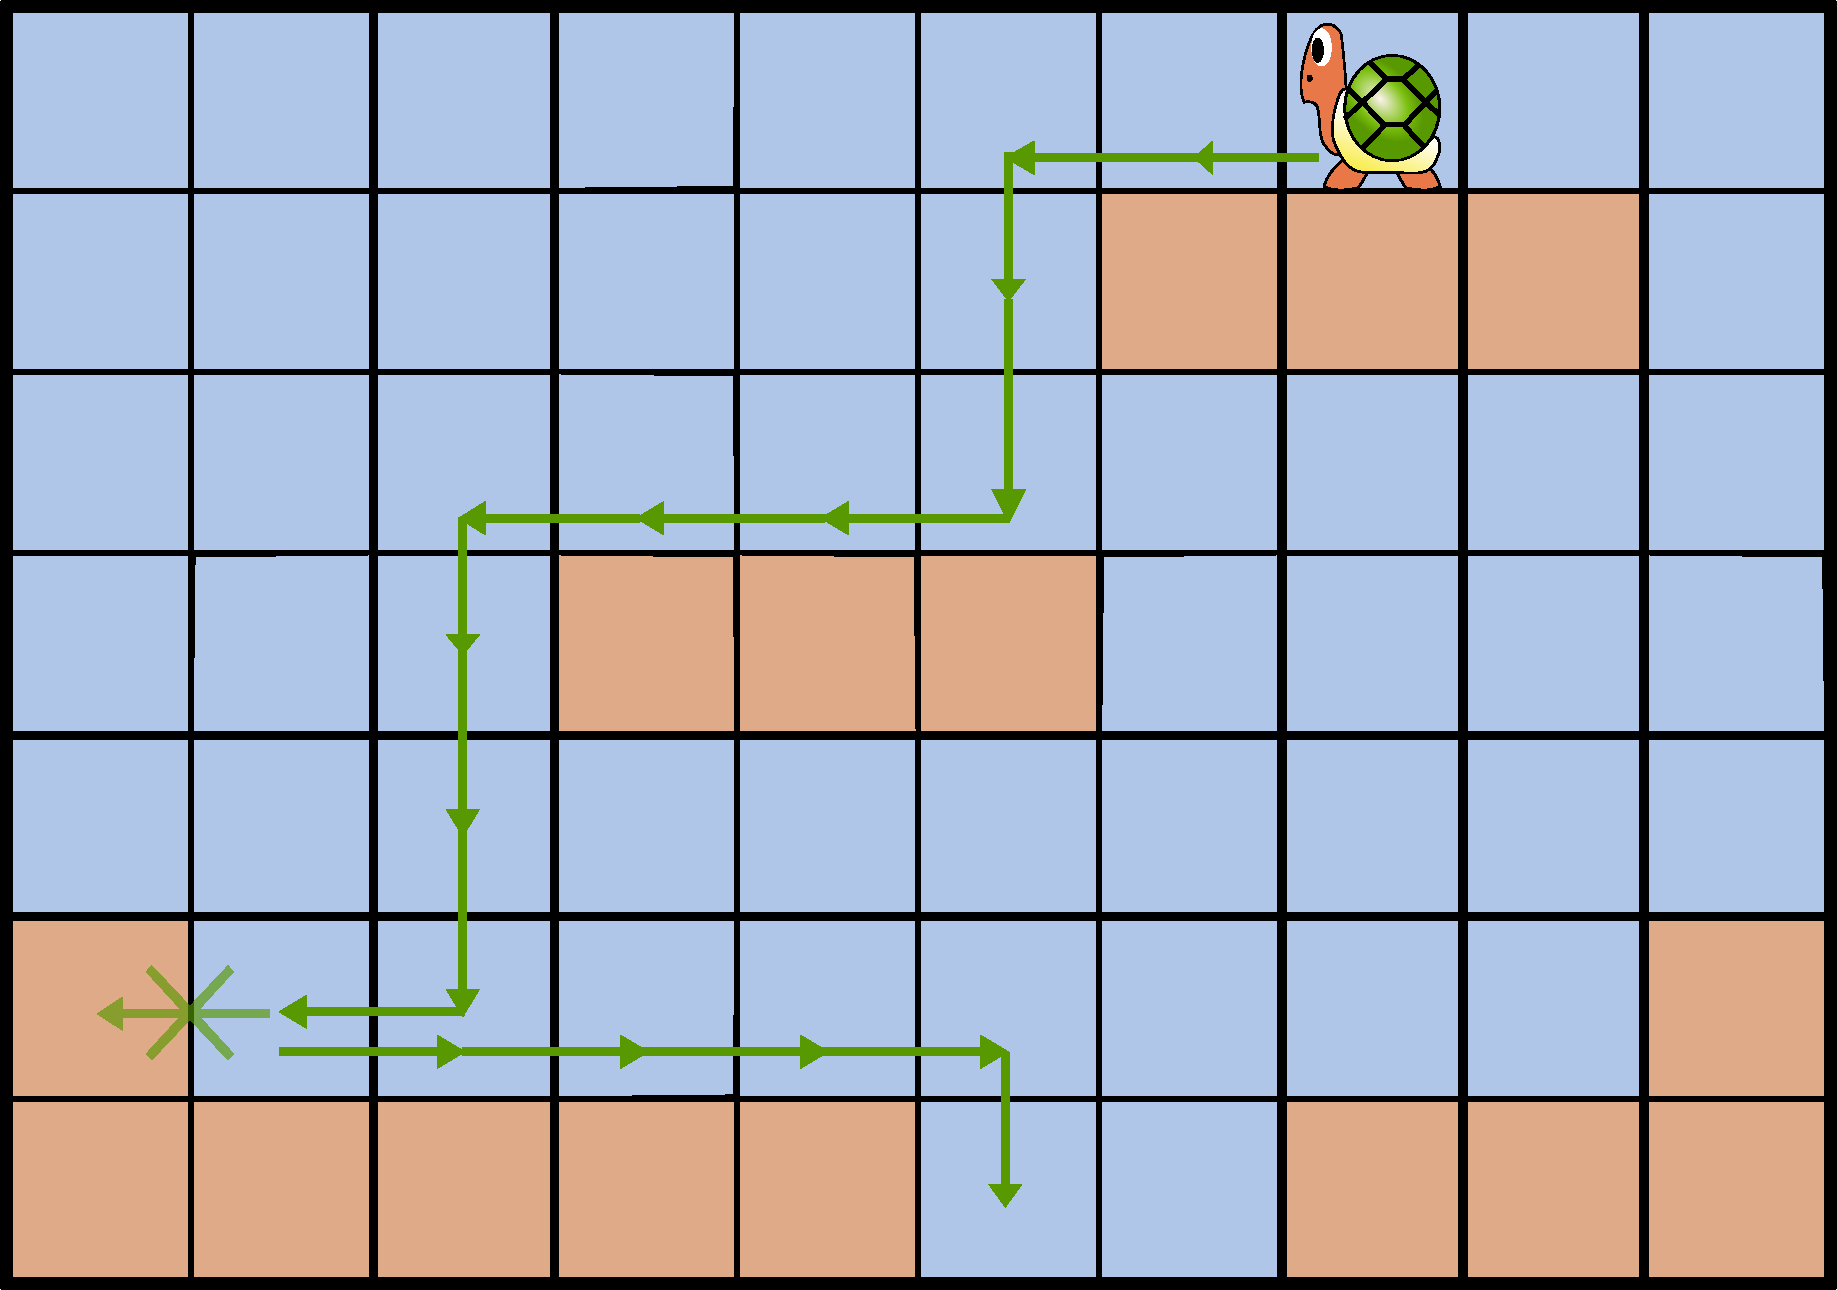
\includegraphics[width=\textwidth]{figures/koopatroopa-green}
  \end{subfigure}
  \caption{Mogelijke paden voor rode en groene Koopa Troopas}
  \label{kooparedgreen}
\end{figure}


\section{Koopa Troopas in Agda}

Om het programmeren met dependent types zo duidelijk mogelijk te illustreren
wordt alle code stap voor stap bekeken in begrijpelijke stukken.  

De code begint met een module declaratie, deze is niet verplicht maar wel
nuttig omdat ze het mogelijk maakt de code te gebruiken in andere programma's.
Daarna importeren we een aantal eenvoudige types uit de standard library.

\inputagda[firstline=8, lastline=15, breaklines]{agda-casestt/koopa.agda}

\iagda{Data.Nat} bevat een unaire voorstelling van natuurlijke getallen die we
gaan gebruiken voor coördinaten. \iagda{Data.Fin} definieert een type voor
begrensde natuurlijke getallen, dit gebruiken we zodat we bij index operaties
niet buiten het bereik van een lijst kunnen gaan. \iagda{Data.Vec} definieert
lijsten met een vaste lengte, vectors dus. \iagda{Data.Unit} definieert een
type, \iagda{⊤} ook wel top genoemd, met één waarde namelijk \iagda{tt}. En,
ten laatste, \iagda{Data.Empty} definieert een leeg type, \iagda{⊥} ook wel
bottom genoemd, waarvoor dus geen waarden bestaan. Dit is anders dan in Haskell
waar je eigenlijk geen leeg type kunt hebben, elk type bevat daar minstens
bottom, wat verschillende dingen kan betekenen, bijvoorbeeld niet eindiging of
een error.

Het volgende stuk is een geneste module declaratie waarin het type
\iagda{Matrix} wordt gedefinieerd als een vector van vectoren en een functie
die een element uit een \iagda{Matrix} projecteert. \iagda{Matrix} is een
inductive family zoals eerder besproken in sectie \ref{sec:indfamagda}. Omdat
\iagda{Matrix} hier gedefinieerd is als een vector van vectoren kunnen we voor
de \iagda{lookup} functie de \iagda{lookup} functies voor vectoren gebruiken.
De volgorde van de indices speelt hierbij een rol maar omdat de indices van het
type \iagda{Fin n} zijn, kan Agda een fout geven als we ze omwisselen.
Vervolgens wordt de module geopend zodat we het type en de functie kunnen
gebruiken zonder de namen te moeten kwalificeren met de naam van de module.

\inputagda[firstline=17, lastline=23, breaklines]{agda-casestt/koopa.agda}

Hierna begint de oplossing van het probleem eigenlijk pas echt. We definiëren
een aantal types waarmee we de Koopa Troopas en de levels kunnen voorstellen.

\inputagda[firstline=25, lastline=30, breaklines]{agda-casestt/koopa.agda}

Koopa Troopas kunnen twee kleuren hebben dus we definiëren een type
\iagda{Color} met een constructor voor elke kleur. Agda laat ons toe om
constructors met hetzelfde type te groeperen als volgt: \iagda{Green Red :
Color}. Het type \iagda{KoopaTroopa} is geïndexeerd op \iagda{Color}, dit wil
dus zeggen dat er een type is voor elke \iagda{Color}. De constructor maakt
gebruik van de Agda syntax voor mixfix notatie, in dit geval is \iagda{_KT} dus
een postfix constructor. De \iagda{_KT} constructor verwacht een \iagda{Color}
en maakt dan een waarde van het type \iagda{KoopaTroopa c} waar die \iagda{c}
dus de waarde van het argument is. Een groene Koopa Troopa kunnen we dus
voorstellen als \iagda{Green KT} en heeft het type \iagda{KoopaTroopa Green},
later wordt duidelijk waarom het belangrijk is dat de kleur in het type zit.

Het volgende stuk bevat nog een aantal type declaraties. Hier definiëren we
posities met alle informatie die we later nodig hebben om te bepalen op welke
posities een Koopa Troopa mag staan.

\inputagda[firstline=32, lastline=48, breaklines]{agda-casestt/koopa.agda}

Elke positie is ofwel lucht, \iagda{gas}, ofwel vast, \iagda{solid}: grond of
muur of iets dergelijks. Het type \iagda{Material} stelt deze toestanden voor.
Het type \iagda{Clearance} gebruiken we om te bepalen wie of wat waar mag
komen. Een positie met \iagda{Clearance} \iagda{Low} kan door eender welke
Koopa Troopa betreden worden maar een positie met \iagda{Clearance}
\iagda{High} kan enkel door groene Koopa Troopas betreden worden en gebruiken
we om posities aan te duiden waar de enige logische beweging vallen is. De
\iagda{Clearance} \iagda{Ultimate} gebruiken we voor posities waar geen enkele
Koopa Troopa mag komen. Een positie stellen we voor door een record met twee
velden voor een horizontale en een verticale coördinaat, een veld dat het
\iagda{Material} van de positie aangeeft en een veld voor de \iagda{Clearance}.
De constructor \iagda{pos} kunnen we gebruiken om een positie op te stellen,
een voorbeeld van een positie kan dus zijn: \iagda{pos 3 5 gas Low}, let
hierbij op dat de cijfers door Agda begrepen worden als natuurlijke getallen,
hiermee kunnen we ook enkel natuurlijke getallen voorstellen.

Om de Koopa Troopas een \iagda{Clearance} te geven moeten we ze op een of
andere manier differentiëren en het enige dat verschilt tussen de Koopa Troopas
is hun kleur wat dus de meest logische bepalende factor van de
\iagda{Clearance} wordt.

\inputagda[firstline=50, lastline=52, breaklines]{agda-casestt/koopa.agda}

In plaats van groen en rood gelijk te stellen aan respectievelijk een hoge en
een lage \iagda{Clearance}, werkt de constructor \iagda{<red>} voor beide
kleuren terwijl \iagda{<green>} enkel voor groen werkt. Dit zorgt ervoor dat we
later niet moeten zorgen dat overal waar een lage \iagda{Clearance} toegelaten
is ook een hoge \iagda{Clearance} toegelaten is, een groene Koopa Troopa krijgt
gewoon de \iagda{Clearance} die hij nodig heeft. We zien hier ook dat de mixfix
notatie even goed voor types te gebruiken is, in dit geval gebruiken we dit om
het type voor te stellen als een pijl, \iagda{_c>_}, van een kleur naar een
\iagda{Clearance}.

De volgende twee definities zijn eigenlijk het belangrijkste deel van de
oplossing en steunen op alle voorgaande concepten.

\inputagda[firstline=54, lastline=61, breaklines]{agda-casestt/koopa.agda}

Het \iagda{_follows_⟨_⟩} type is op het eerste zicht waarschijnlijk een beetje
vreemd, dit is omdat de waarden van het type eigenlijk minder belangrijk zijn
dan het type zelf. Het type drukt uit welke positie kan volgen op welke positie
rekening houdend met een kleur. Omdat hier de types van de constructors
belangrijk zijn, overlopen we ze één voor één. De \iagda{stay} constructor
drukt uit dat een Koopa Troopa altijd kan blijven staan zolang hij in lucht
staat met een lage \iagda{Clearance}. De \iagda{Material} moet \iagda{gas} zijn
omdat een Koopa Troopa niet in grond of muren mag staan en de \iagda{Clearance}
moet \iagda{Low} zijn omdat we willen dat ook rode Koopa Troopas kunnen
stilstaan.  Eigenlijk is stilstaan niet echt een nodige \emph{beweging} maar
hiermee kunnen we later de eindpositie van een pad expliciet maken. De volgende
twee constructors \iagda{next} en \iagda{back} bekijken we tegelijk omdat ze
heel gelijkaardig zijn. Ze drukken uit dat een positie met een bepaalde
\iagda{Clearance} enkel kan volgen op een horizontaal vorige, respectievelijk
volgende, positie als de kleur van de Koopa Troopa die \iagda{Clearance}
oplevert. Ook moet de voorgaande positie een lage \iagda{Clearance} hebben, dit
is omdat we de hoge \iagda{Clearance} gebruiken voor posities waar de enige
mogelijke beweging vallen is. Het \iagda{Material} voor de posities moet nog
steeds \iagda{gas} zijn omdat Koopa Troopas niet in muren kunnen lopen.  De
laatste constructor is \iagda{fall} en die kan enkel gebruikt worden als
beweging van een positie met een hoge \iagda{Clearance}. Aangezien enkel groene
Koopa Troopas op een positie met een hoge \iagda{Clearance} kunnen geraken,
zijn dat ook de enige die kunnen vallen. Nogmaals kunnen we alleen vallen van
een positie in lucht naar een positie in lucht, Koopa Troopas kunnen dus niet
de grond in vallen.

\inputagda[firstline=64, lastline=69, breaklines]{agda-casestt/koopa.agda}

Het type waarmee we de paden voorstellen die Koopa Troopas kunnen afleggen,
\iagda{Path}, moet ervoor zorgen dat enkel geldige paden worden opgesteld voor
een bepaalde Koopa Troopa. De parameter voor de kleur is impliciet omdat die
volgt uit het type van de Koopa Troopa. Verder hangt de geldigheid van een pad
af van de Koopa Troopa en kan een pad maar voor één Koopa Troopa tegelijk
opgesteld worden dus is er een parameter waar we een Koopa Troopa verwachten.
Een pad gaat van een beginpositie naar een eindpositie en die moeten kunnen
variëren voor de verschillende constructors, dus dat zijn indices. De
constructor voor een leeg pad, \iagda{[]}, moet een begin- en een eindpositie
hebben, maar die kunnen we impliciet verkrijgen uit de vorige positie van het
pad en als er geen vorige positie is, uit het verwachte type op de plaats waar
we de constructor gebruiken. De constructor om langere paden op te stellen
maakt weer gebruik van mixfix notatie, de \iagda{infixr} declaratie zorgt
ervoor dat de constructor rechts associatief is, waardoor we minder haakjes
zullen nodig hebben. De constructor verwacht een positie \iagda{p}, een pad van
\iagda{q} naar \iagda{r}, \iagda{qs}, en een bewijs dat \iagda{q} kan volgen op
\iagda{p} voor de kleur van de Koopa Troopa en resulteert in een pad van
\iagda{p} naar \iagda{r}. \iagda{_↠⟨_⟩_} behoudt de geldigheid van een pad door
het argument van het type \iagda{_follows_⟨_⟩} en de enige manier om een pad te
beginnen is met een leeg pad dat sowieso geldig is. Door deze eigenschappen
zijn alle paden geldig bij wijze van constructie.

We kunnen nu paden beginnen opstellen maar een belangrijk probleem is nog dat
de geldigheid van de paden afhangt van een goede bepaling van de
\iagda{Clearance} van elke positie. Wat volgt is eerst een klein voorbeeld van
een pad en daarna een mogelijke oplossing voor een juiste bepaling van de
\iagda{Clearance} voor elke positie.

\inputagda[firstline=71, lastline=74, breaklines]{agda-casestt/koopa.agda}

Om ervoor te zorgen dat de \iagda{Clearance} juist bepaald wordt, gaan we een
functie gebruiken die de regels voor de bepaling van de \iagda{Clearance} van
een positie uitdrukt.

\inputagda[firstline=78, lastline=86, breaklines]{agda-casestt/koopa.agda}

De \iagda{matterToPosVec} functie verwacht twee vectoren van dezelfde lengte
met \iagda{Material}s in en twee coördinaten die aangeven bij welke positie het
eerste \iagda{Material} in de eerste vector hoort. Het resultaat is een vector
van dezelfde lengte met posities in met de juiste coördinaten, de
\iagda{Material}s uit de eerste vector en de juiste \iagda{Clearance} die
afhangt van het \iagda{Material} van de positie onder een positie, vandaar dat
we twee vectoren in de invoer nodig hebben. Het basisgeval is wanneer de
vectoren leeg zijn, in het andere geval bepaalt de functie \iagda{clearance}
wat de juiste \iagda{Clearance} voor de positie is aan de hand van het
\iagda{Material} van de positie zelf en van de positie er onder. Lucht boven
lucht heeft \iagda{Clearance} \iagda{High} omdat daar alleen gevallen kan
worden, lucht boven grond heeft \iagda{Clearance} \iagda{Low} omdat elke Koopa
Troopa moet kunnen staan. Alle grond en muur posities hebben \iagda{Clearance}
\iagda{Ultimate} omdat geen enkele Koopa Troopa zich in een muur of in de grond
mag bevinden.

Door vectoren te geven van alle \iagda{Material}s op een horizontale rij en de
rij daaronder kunnen we nu de \iagda{Clearance}s juist bepalen. Voor de
voorstelling van een level kunnen we dus een vector van zulke vectoren
gebruiken. Uiteindelijk willen we een matrix van posities die het level
voorstelt maar omdat het voor de recursie beter uitkomt als we met een vector
van vectoren werken voor de invoer, gebruiken we geen matrix voor de invoer.

\inputagda[firstline=88, lastline=98, breaklines]{agda-casestt/koopa.agda}

De functie \iagda{matterToPosVecs} maakt gebruik van de vorige functie om een
vector van vectoren van \iagda{Material}s om te zetten in een vector van
vectoren van posities. Het basisgeval is de lege vector en die wordt omgezet in
een lege vector. In het recursieve geval zien we dat de \iagda{_∷_} constructor
voor vectoren gebruikt wordt in de prefix vorm, dit is omdat we willen pattern
matchen op een derde impliciet argument en drie argumenten gaan niet goed samen
met een binaire infix constructor. We gebruiken \iagda{matterToPosVec} op de
eerste vector in de vector van vectoren en op de vector daaronder, die we
verkrijgen uit de functie \iagda{unders}. \iagda{unders} is eigenlijk heel
gelijkaardig aan de \iagda{head} functie maar is specifieker voor een vector
van vectoren en heeft een \emph{fallback} argument dat we teruggeven als we de
rij onder de laatste rij nodig hebben. Het enige dat dan nog rest is om de
recursieve oproep te doen op de rest van de vector van vectoren. De
\iagda{matsToMat} functie maakt van de vector van vectoren van posities, die we
terugkrijgen uit \iagda{matterToPosVecs}, een matrix waarbij de rijen eerst van
volgorde gewisseld worden omdat de index $(0,0)$ bij een matrix linksboven zit
en in de levelvoorstelling links onder.

Met deze functies kunnen we gemakkelijk een level opstellen door de juiste
\iagda{Material}s in de juiste volgorde op te geven, hierbij wordt dan meteen
de juiste \iagda{Clearance} bepaalt voor elke positie. Om onze notatie iets
visueler te maken definiëren we nog twee functies met een unicode symbool.

\inputagda[firstline=100, lastline=114, breaklines]{agda-casestt/koopa.agda}

De functies \iagda{□_} en \iagda{■_} zijn gewoon afkortingen voor
respectievelijk een vector die begint met \iagda{gas} en nog een staart
verwacht en een vector die begint met \iagda{solid} en nog een staart verwacht.
Deze functies zijn gedefinieerd met een underscore ook al zijn ze gewoon prefix
functies omdat de \iagda{infixr} declaratie enkel van toepassing is op mixfix
functies. Zoals we kunnen zien is het level, dat tevens in figuur
\ref{kooparedgreen} te zien is, redelijk herkenbaar ook al stellen we het
gewoon voor met tekst, dit is een voordeel van werken met de volledige unicode
karakterset.

Het enige dat ons nu nog rest te definiëren zijn een aantal hulp functies om
natuurlijke getallen om te zetten in getallen van het type \iagda{Fin n} omdat
we die niet met cijfers kunnen schrijven.

\inputagda[firstline=116, lastline=130, breaklines]{agda-casestt/koopa.agda}

De eerste functie, \iagda{_<'_}, vergelijkt twee natuurlijke getallen en geeft
een type terug, in een taal waar types geen waarden zijn gaat dit meestal niet.
Als het eerste getal strikt kleiner is dan het tweede is dit type \iagda{⊤},
anders is het type \iagda{⊥}. Een element van het type \iagda{⊤} kan altijd
impliciet ingevuld worden, er is er namelijk maar één: \iagda{tt}. Een element
van het type \iagda{⊥} kan nooit gegeven worden want er zijn er geen.  Van deze
functie maken we gebruik in het type van \iagda{fromNat}, een functie die een
natuurlijk getal omzet in een element van \iagda{Fin n}. We kunnen een
natuurlijk getal \iagda{k} maar omzetten in een \iagda{Fin n} als \iagda{k}
strikt kleiner is dan \iagda{n}. Het type \iagda{k <' n} is ofwel gelijk aan
het type \iagda{⊤} ofwel aan het type \iagda{⊥}, in het eerste geval moeten we
dus geen expliciete waarde geven, in het tweede geval kunnen we geen waarde
geven en dus kunnen we de functie ook niet oproepen met een \iagda{k} die we
nooit kunnen omzetten in een \iagda{Fin n}. Op deze manier kan de typechecker
ons waarschuwen wanneer we dit ergens wel proberen te doen. In deze functie
zien we nog iets nieuws, de eerste vergelijking heeft geen rechterzijde. Dit is
omdat er geen waarde bestaat van het type \iagda{Fin 0}, dat isomorf is met het
type \iagda{⊥}. Omdat de \iagda{n} in \iagda{Fin n} een natuurlijk getal is, is
\iagda{0} niet uitgesloten en omdat Agda een totale programmeertaal is moeten
we voor elke mogelijke waarde van het argument \iagda{n} een antwoord bieden.
In dit geval is het type \iagda{k <' n} sowieso gelijk aan \iagda{⊥} en omdat
we geen waarde van dat type kunnen krijgen kunnen we gebruik maken van het
zogenaamde \emph{absurd} pattern: \iagda{{}} of \iagda{()}. Het absurd pattern
geeft aan dat er onmogelijk een waarde van het juiste type bestaat, de
typechecker moet dit wel kunnen nagaan dus dit werkt alleen voor types die
eenvoudig genoeg zijn. Als Agda overtuigd is dat er geen waarde bestaat, moeten
we ook geen rechterzijde opgeven. In de derde vergelijking zien we nog dat het
\emph{bewijs} dat \iagda{k} kleiner is dan \iagda{n} expliciet doorgegeven
wordt en dus geldig blijft voor het recursieve geval, het is tenslotte ook maar
een eenvoudige waarde, \iagda{tt}. De functie \iagda{f} is slechts een
afkorting voor \iagda{fromNat}. De functie \iagda{p} is een afkorting voor
\iagda{lookup} waarbij de coördinaten omgewisseld zijn voor de leesbaarheid en
het level niet moet opgegeven worden omdat dat in alle voorbeelden hetzelfde
is.

Met al deze extra definities kunnen we nu paden op een compacte manier
definiëren zoals we in de rest van de voorbeelden zien.

\inputagda[firstline=132, lastline=144, breaklines]{agda-casestt/koopa.agda}

\iagda{red_path_one} en \iagda{red_path_two} stellen de paden voor die door de
rode Koopa Troopas afgelegd wordt in figuur \ref{kooparedgreen}, het vakje
linksonder heeft coördinaat $(0,0)$, de x-as loopt horizontaal en de y-as
verticaal. Voorbeelden van paden waar niets mis mee is, zijn eigenlijk niet zo
interessant, die kunnen in het originele spel ook voorgesteld worden. Het wordt
pas interessant als we proberen om een ongeldig pad op te stellen, want dat is
wat we proberen te voorkomen.

\inputagda[firstline=1, lastline=12, breaklines]{agda-casestt/koopa-errors.agda}

De fout bij \iagda{red_nopath_one} ziet eruit als volgt:

%----------------------------------------%
\begin{minted}[fontsize=\small]{agda}
  gas != solid of type Material
  when checking that the expression stay has type
  pos 0 (suc zero) gas Low follows p (f 0) (f 1) ⟨ Red ⟩
\end{minted}

Agda geeft aan dat de positie in het type van \iagda{stay} niet overeenkomt met
de positie, door \iagda{stay} te gebruiken op positie $(0,1)$ zou het type
\iagda[breaklines]{pos 0 1 solid Ultimate follows pos 0 1 solid Ultimate ⟨ Red
⟩} moeten zijn maar dat is niet toegelaten in de definitie van de constructor.
Eigenlijk verwachten we een fout, daar waar we een muur in lopen en hier
krijgen we de fout pas te zien als we al in een muur staan. Dit is omdat de
\iagda{_↠⟨_⟩_} constructor rechts associatief is, dus de eerste fout die Agda
tegenkomt, zit zo ver mogelijk vanachter in het pad.

In de fout voor \iagda{red_nopath_two} kunnen we zien dat de beweging waarbij
we een muur zouden inlopen wel als fout wordt gezien:

%----------------------------------------%
\begin{minted}[fontsize=\small]{agda}
  gas != solid of type Material
  when checking that the expression p (f 1) (f 1) ↠⟨ back ⟩ [] has
  type Path (Red KT) (p (f 1) (f 1)) (p (f 0) (f 1))
\end{minted}

Deze fout is zo goed als hetzelfde als de vorige, alleen gaat het nu om de
\iagda{back} constructor en is de expressie waar de fout zich bevindt niet even
ver gereduceerd omdat het type van \iagda{back} ingewikkelder is.

Een pad voor een rode Koopa Troopa moet ook ongeldig zijn als een Koopa Troopa
zou vallen bij het afleggen van het pad:

%----------------------------------------%
\begin{minted}[fontsize=\small]{agda}
  Low != High of type Clearance
  when checking that the expression p (f 4) (f 1) ↠⟨ next ⟩ [] has
  type Path (Red KT) (p (f 4) (f 1)) (p (f 5) (f 1))
\end{minted}

Als een rode Koopa Troopa van een afgrond afloopt, is het niet het
\iagda{Material} dat in de weg zit, het is namelijk allemaal lucht, maar wel
het feit dat een rode Koopa Troopa niet de juiste \iagda{Clearance} heeft.

Voor een groene Koopa Troopa kunnen we opnieuw geldige paden opstellen.

\inputagda[firstline=159, lastline=184, breaklines]{agda-casestt/koopa.agda}

In \iagda{green_path_one} zien we één van de geldige paden voor rode Koopa
Troopas terugkomen. Een pad dat geldig is voor een rode Koopa Troopa is ook
geldig voor een groene Koopa Troopa. In het oorspronkelijke spel zijn Koopa
Troopas ook obstakels voor elkaar, op die manier zou een groene Koopa Troopa
dus beperkt kunnen worden tot een pad dat een rode ook kan afleggen. Evenzeer
is een pad voor een rode Koopa Troopa die omkeert voor er een obstakel in de
weg zit, mogelijk. Opnieuw kan dit nuttig zijn, bijvoorbeeld om de Koopa
Troopas actief de speler te laten achtervolgen als die in de buurt komt,
waarbij ze dus vroeger dan nodig omkeren. In \iagda{green_path_two} zien we het
langere pad dat in figuur \ref{kooparedgreen} geïllustreerd is.

Voor een groene Koopa Troopa is het geen fout als het pad van een afgrond af
gaat en dan naar beneden valt. Maar er treedt zoals verwacht nog wel een fout
op als we proberen een muur in te lopen.

\inputagda[firstline=14,lastline=16,breaklines]{agda-casestt/koopa-errors.agda}

%----------------------------------------%
\begin{minted}[fontsize=\small]{agda}
  gas != solid of type Material
  when checking that the expression p (f 1) (f 1) ↠⟨ back ⟩ [] has
  type Path (Green KT) (p (f 1) (f 1)) (p (f 0) (f 1))
\end{minted}

Deze fout is identiek aan die voor \iagda{red_nopath_two}. In het volgende deel
bespreken we de implementatie van dit model in Haskell.


\section{Koopa Troopas in Haskell}

In Haskell beginnen we de code met de LANGUAGE pragma's die besproken zijn in
hoofdstuk \ref{ch:agda-haskell}. Daarna komt de module declaratie, hier zien we
voor de eerste keer dat Haskell redelijk strikte regels heeft over naamgeving,
modules types en constructors moeten met een hoofdletter beginnen en functies
met een kleine letter.

\inputhaskell[firstline=8, lastline=11, breaklines]{haskell-casestt/koopa.hs}

Om te beginnen moeten we een aantal types die we in Agda uit de standard
library kunnen halen zelf implementeren or is bijvoorbeeld geen erg grote nood
aan een unaire voorstelling van natuurlijke getallen in Haskell. De naamgeving
en technieken die we hier gebruiken komen uit een artikel \cite{hasochism} over
dependently typed programmeren in Haskell met de titel: "Hasochism: The
Pleasure and Pain of Dependently Typed Haskell Programming." Het wordt redelijk
snel duidelijk waarom het artikel die titel heeft.

\inputhaskell[firstline=13, lastline=24, breaklines]{haskell-casestt/koopa.hs}

We beginnen met het definiëren van onze unaire natuurlijke getallen, dankzij de
datatype promotion van de DataKinds extensie hebben we nu ook meteen unaire
natuurlijke getallen op het typeniveau. Wat we nog missen is een verbinding
tussen waarden op het waardeniveau en waarden op het typeniveau zoals die er
wel is in Agda, daar kunnen we een argument van de functie ook in het type
gebruiken. In Haskell kunnen we dit niet echt doen, maar we kunnen het wel
imiteren met een zogenaamde singleton constructie. Dit zien we in de definitie
van \ihask{Natty}, elke waarde die we opstellen heeft een ander type:
\ihask{Zy} heeft type \ihask{Natty Z} en \ihask{Sy Zy} heeft type \ihask{Natty
(S Z)}. Omdat elk type \ihask{Natty n} maar één waarde bevat, heeft deze
constructie de benaming singleton gekregen. De functie \ihask{natter}, ongeveer
te lezen als "meer Nat-achtig," zet een \ihask{Natty n} om in een \ihask{Nat},
hierbij werpen we als het ware informatie op het typeniveau weg. De omgekeerde
conversie gaat niet zomaar, er is geen manier om statisch te bepalen wat de
\ihask{n} in het return type \ihask{Natty n} zou moeten zijn. Om dit bij
benadering toch te kunnen doen hebben we een derde type nodig, \ihask{NATTY}.
Dit type verstopt als het ware de typeniveau informatie van een \ihask{Natty
n}. Nu kunnen we de functie \ihask{nattyer}, "meer Natty-achtig," wel
schrijven. De definitie is eenvoudig, in het recursieve geval moeten we een
pattern match doen op de recursieve oproep om met de eigenlijke waarde van de
\ihask{Natty} te kunnen werken.

Haskell ontbreekt logischerwijs tevens een type voor begrensde natuurlijke
getallen. Deze keer kunnen we de extra types niet definiëren omdat Haskell het
\ihask{Fin} type niet kan promoveren. De DataKinds extensie promoveert enkel
types met argumenten met \emph{kind} \ihask{*} en \ihask{Fin} heeft een argument met
\emph{kind} \ihask{Nat}.

\inputhaskell[firstline=27, lastline=35, breaklines]{haskell-casestt/koopa.hs}

De definitie voor \ihask{Fin} is identiek aan die uit de Agda standard library
voor zover dat mogelijk is. De functie \ihask{intToFin} dient ongeveer
hetzelfde doel als de \iagda{fromNat} functie uit de Agda code. Omdat Haskell
geen cijfers toelaat voor natuurlijke getallen, vertrekken we van het
\ihask{Integer} type. Dit brengt met zich mee dat we negatieve getallen
toelaten, hiervoor werpen we gewoon een fout op.

Vervolgens is er het type \ihask{Vec} dat ook weer logischerwijs niet in
Haskell aanwezig is met de bijhorende functies.

\inputhaskell[firstline=38, lastline=58, breaklines]{haskell-casestt/koopa.hs}

Haskell laat binaire infix constructors toe door hun naam te beginnen met een
dubbelpunt, toevallig kunnen we zo bijna dezelfde notatie gebruiken als in
Agda. \ihask{vlookup} haalt een element uit een vector met behulp van een
begrensd getal dus we sluiten uit dat een index te groot of te klein is.
\ihask{vreplicate} stelt een vector op met een bepaald aantal herhalingen van
een element, we hebben hier een \ihask{Natty n} nodig omdat we de waarde
\ihask{n} moeten kennen voor het type van de vector die we willen teruggeven.
\ihask{vreverse} keert de volgorde van de elementen in een vector om.

Nu kunnen we ook het \ihask{Matrix} type definiëren. Dit type en de voorgaande
types zijn niet gedefinieerd in submodules zoals we \iagda{Matrix} gedefinieerd
hebben in Agda omdat Haskell geen concept heeft van submodules. We zouden deze
types allemaal in modules in hun eigen bestanden kunnen definiëren maar omdat
het weinig code is en slechts tot voorbeeld dient, is dit achterwege gelaten.

\inputhaskell[firstline=61, lastline=65, breaklines]{haskell-casestt/koopa.hs}

Zowel het \ihask{Matrix} type als de \ihask{mlookup} functie gelijken sterk op
hun tegenhangers in Agda. Het grootste verschil is dat we in Haskell met
polymorfisme werken daar waar we in Agda gewoonlijk impliciete argumenten
gebruiken.

Voor het \ihask{Color} type hebben we weer het type zelf en een singleton type
nodig, \ihask{Colorry}, omdat we in het \ihask{KoopaTroopa} type de kleur uit
het argument nodig hebben op het typeniveau.

\inputhaskell[firstline=67, lastline=73, breaklines]{haskell-casestt/koopa.hs}

Wat we hierbij ook kunnen opmerken is dat het type \ihask{KoopaTroopa}
eigenlijk hetzelfde is als \ihask{Colorry} op de constructors na, en hier zit
het probleem: als we een constructor willen die een kleur argument neemt en
gebruik maakt van de bijhorende waarde op het typeniveau moet dat argument een
singleton type hebben.

Voor de \ihask{Material} en \ihask{Clearance} types hebben we dezelfde
constructies nodig als voor de natuurlijke getallen.

\inputhaskell[firstline=75, lastline=95, breaklines]{haskell-casestt/koopa.hs}

Het veelvoud aan types dat we op deze manier krijgen is conceptueel geen
probleem maar praktisch is het wel lastig. Soms hebben we een waarde van het
ene type en hebben we één van de andere types nodig dus moeten we een functie
gebruiken om van een \ihask{Matty} een \ihask{Material} te maken, jammer genoeg
gaat deze omzetting niet altijd in de omgekeerde richting. Om de omzetting van
\ihask{Material} naar \ihask{Matty} toch te doen hebben we het type
\ihask{MATTY} maar bij deze omzetting verliezen we de informatie op het
typeniveau waarvoor we \ihask{Matty} net gemaakt hebben. Dit is niet altijd een
probleem maar komt wel voortdurend terug als we met deze constructies werken.

Omdat we in het type voor een pad gebruik willen maken van de waarden van de
posities, hebben we voor posities weer dezelfde constructie nodig, alleen is
deze nu uitgebreider.

\inputhaskell[firstline=98, lastline=114, breaklines]{haskell-casestt/koopa.hs}

In de functie \ihask{positionnyer} zien we een geval waar
we de waarden uit de types \ihask{NATTY}, \ihask{MATTY} en \ihask{CLEARRY}  als
het ware kunnen uitpakken, dit is alleen mogelijk omdat we ze daarna terug
inpakken in een waarde met type \ihask{POSITIONNY}.

Het volgende concept dat we moeten uitdrukken is de relatie tussen een kleur en
de bijhorende \ihask{Clearance}, in Agda gebruiken we hiervoor een type en
instance arguments. Omdat we niet telkens expliciet een waarde willen meegeven
die toch niet gebruikt wordt, wat we gebruiken is immers het type, gebruiken we
een typeclass in Haskell.

\inputhaskell[firstline=116,lastline=118,breaklines]{haskell-casestt/koopa.hs}

Op deze manier kunnen we met een typeclass constraint aan de informatie geraken
die we nodig hebben zonder een expliciet argument.

Voor het \ihask{Follows} type is de implementatie redelijk eenvoudig. Buiten de
typeclass constraint in plaats van een instance argument en het polymorfisme in
plaats van impliciete argumenten, is het grootste verschil de syntax. Haskell
laat binaire infix constructors toe en met de extensie TypeOperators
\cite{typeops} ook types en typeclasses maar een ternaire mixfix notatie is er
niet. We gebruiken dus gewoon een type met drie parameters.

\inputhaskell[firstline=120,lastline=124,breaklines]{haskell-casestt/koopa.hs}

Voor het type \ihask{Path} komen we een probleem tegen.

\inputhaskell[firstline=126,lastline=128,breaklines]{haskell-casestt/koopa.hs}

\ihask{Path} kan geen parameter hebben met \emph{kind} \ihask{KoopaTroopa} omdat het
type \ihask{KoopaTroopa} een parameter heeft met een \emph{kind}, namelijk
\ihask{Color}, dat niet \ihask{*} is. Zo'n type kan door de DataKinds extensie
niet gepromoveerd worden dus kunnen we het ook niet als \emph{kind} gebruiken.

Op dit punt kunnen we hetzelfde pad voorstellen als in de Agda code.

\inputhaskell[firstline=133,lastline=136,breaklines]{haskell-casestt/koopa.hs}

\ihask{exPath} is heel gelijkaardig aan \iagda{ex_path} uit Agda maar de unaire
voorstelling die we moeten gebruiken voor de getallen doet wel afbreuk aan de
leesbaarheid.

De functies om een \ihask{Matrix} op te stellen aan de hand van een vector van
vectoren van \ihask{Material}s zijn redelijk eenvoudig. We hebben wel
expliciete argumenten nodig voor de breedte en hoogte maar eigenlijk om een
andere reden dan vorig gebruiken van de singleton types. In dit geval hebben we
de informatie al op het typeniveau en hebben we ze in \ihask{matterToPosVecs}
nodig op het niveau van waarden. De enige manier om dit te bereiken is met
expliciete argumenten van een singleton type.

\inputhaskell[firstline=138,lastline=163,breaklines]{haskell-casestt/koopa.hs}

De enige functies uit Agda die we nog missen in Haskell zijn de functies die
een \ihask{Material} voorstellen met een symbool. In Haskell kunnen we deze wel
definiëren zoals in Agda, mits we geldige karakters gebruiken, functienamen
moeten uit alfanumerieke karakters bestaan en niet alle unicode karakters zijn
alfanumeriek. Maar omdat we geen fixity declaratie kunnen geven voor een
functie en geen unaire operatoren kunnen definiëren, is er geen manier om deze
functies rechts associatief te maken. Als we de constructor \ihask{(:>)} dus
mee zouden opnemen in de functies zouden we overal \ihask{\$} moeten gebruiken
waar nu de constructor staat.

\inputhaskell[firstline=165,lastline=168,breaklines]{haskell-casestt/koopa.hs}

Het voorbeeld level ziet er hetzelfde uit ook al is dit minder duidelijk door
de symbolen die we gebruiken.

\inputhaskell[firstline=170,lastline=183,breaklines]{haskell-casestt/koopa.hs}

De laatste functies die we nog niet gedefinieerd hebben zijn de functies om
onze notatie van de voorbeelden te verkorten.

\inputhaskell[firstline=186,lastline=200,breaklines]{haskell-casestt/koopa.hs}

Omdat we de bovengrens niet impliciet kunnen laten voor \ihask{intToFin},
definiëren we twee functies met de juiste grenzen voor horizontale en verticale
coördinaten, \ihask{ix} en \ihask{iy}. De \iagda{p} functie uit Agda zorgt voor
een probleem in Haskell. Deze functie zou namelijk een \ihask{Positionny p}
moeten teruggeven maar in de \ihask{Matrix} die het level voorstelt zitten
enkel \ihask{Position}s. We weten dat de omzetting van \ihask{Position} naar
\ihask{Positionny} niet zomaar kan en dat we dus een \ihask{POSITIONNY} moeten
teruggeven. Het probleem hiermee duikt pas op in de voorbeelden: we kunnen een
\ihask{POSITIONNY} uitpakken om te werken met de \ihask{Positionny} die erin
zit zolang we die \ihask{Positionny} ofwel verbruiken in een functie, ofwel
terug verpakken in een type zoals \ihask{POSITIONNY}. In \ihask{p} kunnen we
geen van beide doen, het \ihask{Path} heeft de \ihask{Positionny} nodig dus we
kunnen die niet omzetten in iets anders en het type \ihask{Path} heeft ook de
informatie uit het type van de \ihask{Positionny} nodig en daar kunnen we niet
aan.

Dit probleem is wel op te lossen maar de oplossing is niet eenvoudig. Het
probleem is eigenlijk dat we het type van een element niet uit de
\ihask{Matrix} kunnen halen zoals in Agda. Om dit in Haskell te kunnen doen zou
het type \ihask{Matrix} een overeenkomstig singleton type moeten hebben. Maar
\ihask{Matrix} heeft parameters met \emph{kind} \ihask{Nat} en kan dus niet
gepromoveerd worden. Dit kunnen we oplossen door natuurlijke getallen te
definiëren met \emph{kind} \ihask{*}: een leeg type \ihask{Z} en een leeg type
\ihask{S n} bijvoorbeeld. Maar we komen hetzelfde probleem tegen in het type
van de constructor \ihask{Mat}, het vector type daar is ook niet te promoveren
omdat \ihask{Vec} weer een parameter van \emph{kind} \ihask{Nat} heeft. Dit kunnen we
oplossen door het \emph{kind} \ihask{Nat} in de definitie van \ihask{Vec} te vervangen
door het \emph{kind} \ihask{*}. Op deze manier kan de DataKinds extensie het
\ihask{Matrix} type promoveren en kunnen we er een singleton voor definiëren.
Dit is nog niet de hele oplossing en ze is ook niet geïmplementeerd omdat we
hierbij gedeeltelijk garanties verliezen. Plotseling is \ihask{S Bool} een
geldig type en \ihask{Vec Z Char} ook. We zijn dus als het ware \emph{unkinded}
aan het programmeren, analoog aan untyped.

Om dit probleem te omzeilen definiëren we een aantal \ihask{Positionny}s alsof
we ze uit de \ihask{Matrix} voor het voorbeeld level hebben gehaald.

\inputhaskell[firstline=203,lastline=222,breaklines]{haskell-casestt/koopa.hs}

Met deze posities kunnen we alle voorbeelden die we hadden uitdrukken in
Haskell.

\inputhaskell[firstline=224,lastline=240,breaklines]{haskell-casestt/koopa.hs}

De paden komen overeen met die in de Agda code. Net zoals in Agda is het geen
verassing dat we geldige paden kunnen uitdrukken. Het is interessanter om te
kijken naar de fout die we krijgen bij de ongeldige paden.

\inputhaskell[firstline=1,lastline=21,
              breaklines]{haskell-casestt/koopa-errors.hs}

De fout voor \ihask{redNoPathOne} is een stuk langer dan die voor
\iagda{red_nopath_one}, dit heeft onder andere te maken met het ontwerp van
Agda. Agda is eigenlijk gemaakt om interactief te werken met de typechecker
terwijl Haskell eerder los van het schrijven wordt gecompileerd. Agda stopt bij
de eerste fout die de typechecker tegenkomt terwijl Haskell doorgaat en
probeert alle fouten te vinden.

%----------------------------------------%
\begin{Verbatim}[fontsize=\small]
  koopa.hs:246:16:
      Couldn't match type 'Gas with 'Solid
      Expected type: Path
                       'Red
                       ('Pos ('S 'Z) ('S 'Z) 'Gas 'Low)
                       ('Pos 'Z ('S 'Z) 'Solid 'Ultimate)
        Actual type: Path
                       'Red ('Pos ('S 'Z) ('S 'Z) 'Gas 'Low)
                            ('Pos 'Z ('S 'Z) 'Gas 'Low)
      In the expression: Pcons p11 Back $ Pcons p01 Stay P0
      In an equation for `redNoPathOne':
          redNoPathOne = Pcons p11 Back $ Pcons p01 Stay P0

  koopa.hs:247:22:
      Couldn't match type 'Solid with 'Gas
      Expected type: Positionny ('Pos 'Z ('S 'Z) 'Gas 'Ultimate)
        Actual type: Positionny ('Pos 'Z ('S 'Z) 'Solid 'Ultimate)
      In the first argument of `Pcons', namely `p01'
      In the second argument of `($)', namely `Pcons p01 Stay P0'
      In the expression: Pcons p11 Back $ Pcons p01 Stay P0

  koopa.hs:247:26:
      Couldj't match type 'Low with 'Ultimate
      Expected type: Follows
                       ('Pos 'Z ('S 'Z) 'Gas 'Low)
                       ('Pos 'Z ('S 'Z) 'Gas 'Ultimate) 'Red
        Actual type: Follows
                       ('Pos 'Z ('S 'Z) 'Gas 'Low)
                       ('Pos 'Z ('S 'Z) 'Gas 'Low) 'Red
      In the second argument of `Pcons', namely `Stay'
      In the second argument of `($)', namely `Pcons p01 Stay P0'
      In the expression: Pcons p11 Back $ Pcons p01 Stay P0
\end{Verbatim}

De eerste fout gaat over het pad als een geheel en zegt dat het eigenlijke
\ihask{Material}, \ihask{Solid}, niet overeenkomt met wat het moet zijn,
\ihask{Gas}. De tweede fout zegt eigenlijk hetzelfde maar dan over de
specifieke positie, Haskell leidt wel af dat de \ihask{Material} \ihask{Gas}
moet zijn maar niet dat de \ihask{Clearance} \ihask{Ultimate} niet zou mogen
voorkomen. De derde fout gaat wel over de \ihask{Clearance} voor een rode Koopa
Troopa. Deze drie zijn heel volledig maar we moeten wel goed opletten dat die
fouten niet allemaal dezelfde oorzaak hebben, zoals hier. Merken we ook nog op
dat de eerste fout alleen verschijnt als we de type signature voor
\ihask{redNoPathOne} geven. We moeten dus goed oppassen met inferentie omdat we
op die manier wel eens iets anders kunnen schrijven dan we bedoelen.

De fout voor \ihask{redNoPathTwo} is veel korter.

%----------------------------------------%
\begin{Verbatim}[fontsize=\small]
  koopa.hs:254:31:
      Couldn't match type 'Gas with 'Solid
      Expected type: Path
                       'Red
                       ('Pos 'Z ('S 'Z) 'Gas 'Ultimate)
                       ('Pos 'Z ('S 'Z) 'Solid 'Ultimate)
        Actual type: Path
                       'Red
                       ('Pos 'Z ('S 'Z) 'Gas 'Ultimate)
                       ('Pos 'Z ('S 'Z) 'Gas 'Ultimate)
      In the third argument of `Pcons', namely `P0'
      In the expression: Pcons p11 Back P0
      In an equation for `redNoPathTwo': redNoPathTwo = Pcons p11 Back P0
\end{Verbatim}

Opnieuw komt het \ihask{Material} dat we verwachten in de type signature niet
overeen met het type dat door \ihask{Pcons} wordt afgedwongen. Als we de type
signature niet opgeven krijgen we ook weer een andere fout.

De fout voor \ihask{redNoPathThree} is nog korter en is ook anders dan de
vorige fouten die allemaal ongeveer hetzelfde waren.

%----------------------------------------%
\begin{Verbatim}[fontsize=\small]
  koopa.hs:262:28:
      No instance for (CoClr 'Red 'High) arising from a use of `Next'
      Possible fix: add an instance declaration for (CoClr 'Red 'High)
      In the second argument of `Pcons', namely `Next'
      In the expression: Pcons p41 Next P0
      In an equation for `redNoPathThree':
          redNoPathThree = Pcons p41 Next P0
\end{Verbatim}

Deze keer heeft de fout niets met \ihask{Material}s te maken maar wel met de
\ihask{Clearance} zoals verwacht. De rode Koopa Troopa heeft geen
\ihask{Clearance} \ihask{High} dus de juiste instance kan niet gevonden worden.
De oplossing die Haskell voorstelt is wel fout, het was een bewuste keuze om
die instance niet te definiëren voor rode Koopa Troopas. Om dit soort
verwarrend advies te vermijden zouden gesloten typeclasses nuttig zijn.

We kunnen ook geldige paden voor groene Koopa Troopas opgeven met dezelfde
opmerkingen als bij de code in Agda: elk pad dat geldig is voor een rode Koopa
Troopa is ook geldig voor groene Koopa Troopas.

\inputhaskell[firstline=264,lastline=294,breaklines]{haskell-casestt/koopa.hs}

Ten slotte is er nog het foute pad voor een groene Koopa Troopa.

\inputhaskell[firstline=23, lastline=27,
              breaklines]{haskell-casestt/koopa-errors.hs}

Met dezelfde fout als voor \ihask{redNoPathTwo}.

%----------------------------------------%
\begin{Verbatim}[fontsize=\small]
  koopa.hs:300:33:
      Couldn't match type 'Gas with 'Solid
      Expected type: Path
                       'Green
                       ('Pos 'Z ('S 'Z) 'Gas 'Ultimate)
                       ('Pos 'Z ('S 'Z) 'Solid 'Ultimate)
        Actual type: Path
                       'Green
                       ('Pos 'Z ('S 'Z) 'Gas 'Ultimate)
                       ('Pos 'Z ('S 'Z) 'Gas 'Ultimate)
      In the third argument of `Pcons', namely `P0'
      In the expression: Pcons p11 Back P0
      In an equation for `greenNoPathOne':
          greenNoPathOne = Pcons p11 Back P0
\end{Verbatim}


\section{Besluit}

We hebben een voorbeeld gezien van wat het is om met dependent types te
programmeren. Voor de garanties die we krijgen van de statische verificatie
betalen we vooral in de omvang van de code. Voor een spel zoals Mario is dit
gewoonlijk niet de moeite maar er zijn genoeg voorbeelden waar statische
verificatie wel die extra moeite waard is. We kunnen bijvoorbeeld  denken aan
applicaties in de ruimtevaart of productie van geïntegreerde circuits
waar een fout in de programmatuur ontzettend duur kan zijn. Of een
veiligheidssysteem waar levens van afhangen. Enkel voor zulke systemen is het
extra werk voor een volledige statische verificatie aanvaardbaar. Maar
dependent types laten toe om maar gedeeltelijke verificatie te doen,
bijvoorbeeld werken met vectoren, in plaats van lijsten en begrensde getallen
als indices, voorkomt elke vorm van indexeringsfouten.

We hebben ook een duidelijk verschil gezien tussen programmeren in een
\emph{volwaardige} dependently type taal en een eerder praktische taal met een
typesysteem dat aan expressiviteit wint. Ik denk dat de titel van het artikel
over dependently type programmeren in Haskell ondertussen wel duidelijk is.
Haskell zit al redelijk dicht bij dependent types maar verschilt nog genoeg om
het heel moeilijk te maken om op deze manier te werken. In Haskell kan het
extra werk nog steeds aanvaardbaar zijn afhankelijk van de kost van fouten maar
is het waarschijnlijk eerder voordelig om te werken met gedeeltelijke
verificatie. Wat hier wel tegenover staat is dat Haskell met deze technieken in
de praktijk bruikbaar is, daar waar Agda nog een lange weg te gaan heeft
voordat dit het geval is. Ook is een ontwikkeling als het singleton package
\cite{singletonpack} het vermelden waard, dit zou gedeeltelijk voor een
vereenvoudiging kunnen zorgen wat de veelheid aan types betreft die we
momenteel nodig hebben.

De code voor dit hoofdstuk is in zijn geheel terug te vinden in bijlagen
\ref{app:case-koopa-agda} en \ref{app:case-koopa-haskell}. In het volgende
hoofdstuk bekijken we een tweede gevalstudie waar we de tekortkomingen van
Haskell tegenover volwaardige dependent types op een andere manier oplossen.

